\documentclass[manuscript]{acmart}

\setcopyright{none}
\citestyle{acmauthoryear}
\raggedbottom
\setlength{\textfloatsep}{8pt plus 2pt minus 2pt}
\setlength{\floatsep}{8pt plus 2pt minus 2pt}
\setlength{\intextsep}{8pt plus 2pt minus 2pt}
\usepackage{tikz}

\acmConference[CI 2026]{ACM Collective Intelligence 2026}{September 27--30, 2026}{Virginia Tech Institute for Advanced Computing, near Washington, DC, USA}
\acmYear{2026}
\acmBooktitle{Proceedings of ACM Collective Intelligence 2026 (CI 2026)}

\begin{document}

\title[Legislative Mechanism Bundles]{A Reproducible Simulation Framework for Comparing Legislative Mechanism Bundles}
\subtitle{Stress Tests for Productivity, Revision Moderation, Public Support, and Risk}

\author{Anonymous Author(s)}
\renewcommand{\shortauthors}{Anonymous Author(s)}
\authorsaddresses{}

\begin{abstract}
Legislatures need enough productivity to act, but productivity alone can also mean volatility, agenda capture, or weakly supported lawmaking. This paper presents a reproducible computational framework for comparing selected legislative mechanism bundles under shared synthetic assumptions. The simulator routes the same generated legislatures and bill streams through legislative-style processes that vary agenda access, proposal revision, voting thresholds, alternative selection, public review, lobbying safeguards, affected-group protection, package bargaining, and reversibility.

The contribution is methodological: a reusable experimental architecture for diagnosing how legislative collective decision mechanisms shift the relationship among throughput, moderating revision, support, risk, and procedural cost under controlled synthetic worlds. The framework is designed to make tradeoffs inspectable rather than to rank real institutions. It reports a diagnostic dashboard separating productivity, revision moderation, public support, low-public-support enactment, risk control, administrative feasibility, and generated public benefit per submitted proposal. A main comparison campaign demonstrates how these metrics separate across representative mechanism families, while scripted diagnostics generate seed, ablation, manipulation-stress, chamber-structure, and empirical boundary checks. The reported results are synthetic, generator-dependent design hypotheses.
\end{abstract}

\begin{CCSXML}
<ccs2012>
<concept>
<concept_id>10003120.10003121.10003124.10010392</concept_id>
<concept_desc>Human-centered computing~Collaborative and social computing theory, concepts and paradigms</concept_desc>
<concept_significance>500</concept_significance>
</concept>
<concept>
<concept_id>10010147.10010257</concept_id>
<concept_desc>Computing methodologies~Modeling and simulation</concept_desc>
<concept_significance>500</concept_significance>
</concept>
<concept>
<concept_id>10010405.10010455.10010460</concept_id>
<concept_desc>Applied computing~Law</concept_desc>
<concept_significance>300</concept_significance>
</concept>
</ccs2012>
\end{CCSXML}

\ccsdesc[500]{Human-centered computing~Collaborative and social computing theory, concepts and paradigms}
\ccsdesc[500]{Computing methodologies~Modeling and simulation}
\ccsdesc[300]{Applied computing~Law}

\keywords{legislative institutions, institutional design, computational simulation, agenda control, revision moderation, collective decision making, voting systems}

\maketitle

\section{Introduction}

The motivating question is whether systematic comparison can distinguish legislative structures that merely pass bills from those that combine productivity, revision, and representative responsiveness. A legislature can be unified without being democratic; authoritarian systems can appear cohesive because disagreement is suppressed. In this framework, representative responsiveness is operationalized through generated public support, generated public benefit, revision behavior, and burden diagnostics for affected groups.

The central modeling choice is to treat final passage thresholds as only one part of a larger institutional process that includes proposal access, agenda control, revision, review, and correction. Burden-shifting passage rules are included only as stress tests because they expose how proposal access, objection rights, information, and correction interact with final voting thresholds.

This paper treats legislative institutions as collective intelligence architectures: procedural rules determine who can contribute proposals, which signals are amplified, how expertise and public support enter decisions, how disagreement is resolved, and how errors are corrected. The simulator is therefore not a forecast of Congress but a tool for comparing institutional aggregation mechanisms under shared synthetic conditions.

The paper contributes four linked artifacts: a modular simulator for legislative mechanism bundles; a diagnostic dashboard separating productivity, support, risk, revision, and cost; a reproducible comparison campaign over selected mechanism families; and stress tests showing how generator assumptions, vote-kernel assumptions, and bounded manipulation probes affect the displayed tradeoffs.

The paper asks three questions. First, can a modular simulator distinguish throughput-producing rules from rules that produce moderated, broadly supported revisions under shared synthetic assumptions? Second, which mechanism families remain relevant when productivity, revision moderation, public support, risk, and administrative burden are evaluated separately? Third, which findings survive sensitivity checks on assumptions, mechanism ablations, and manipulation stressors?

This paper should be read as a framework and stress-test study, not as a validated model of Congress or a recommendation for constitutional reform. The reported results compare institutional mechanisms under shared synthetic assumptions. Empirical held-out and flow smoke tests screen for gross implausibility, but bill-topic opinion, affected-group evidence, bill-specific finance/lobbying influence, implementation outcomes, direct court/statute review, emergency court review, full statutory lineage, and cross-national institutional validation remain future work.

\section{Related Work}

The model draws on individual-level simulation, spatial voting, and institutional theory. Agent-based and computational political models are useful when heterogeneous actors interact under rules that create aggregate outcomes \citep{Epstein2006,GilbertTroitzsch2005,deMarchiPage2014}. Spatial voting motivates one-dimensional ideal points and status-quo-relative utility \citep{Downs1957}. Legislative bargaining and agenda-setter models motivate explicit proposer identity and proposer gain \citep{BaronFerejohn1989,RomerRosenthal1978}. Pivotal-politics and veto-player theories motivate comparing simple majority, supermajority, bicameral, and executive-veto systems \citep{Krehbiel1998,Tsebelis2002}. Committee and agenda-control theory motivates treating floor denial, referral, information, and amendment control as outcomes rather than missing observations \citep{CoxMcCubbins2005,GilliganKrehbiel1987,Krehbiel1991,Shepsle1979,ShepsleWeingast1987,WeingastMarshall1988}.

Several tested mechanisms come from adjacent literatures. Lobbying is modeled as access, effort, information, public pressure, and participation bias rather than only direct vote buying \citep{AustenSmith1993,AustenSmith1995,HallDeardorff2006,HallWayman1990,deFigueiredoRichter2014,GilensPage2014}. Citizen-panel variants draw on deliberative polling and mini-public practice \citep{Fishkin2009,OECD2020}. Agenda-credit variants echo quadratic-voting and storable-vote work on expressing intensity under scarcity \citep{Casella2005,LalleyWeyl2018}. Reversibility variants draw on temporary legislation and sunset review \citep{Gersen2007,Ranchordas2014}. Policy tournaments draw on Condorcet and agenda-manipulation problems \citep{McKelvey1976,Tideman1987}. Model documentation follows ODD and ODD+D conventions \citep{Grimm2010,Muller2013}. In collective intelligence terms, legislatures combine proposal generation, information filtering, preference aggregation, deliberative revision, and error correction. Existing legislative models often isolate one stage; this framework treats the stages as an interacting architecture. This paper contributes an executable comparison environment that treats institutional design as a modular collective intelligence architecture: the same synthetic actors and proposal streams are passed through different agenda, revision, voting, review, and correction mechanisms so diagnostic tradeoffs become inspectable.

\section{Simulator}

Each run creates a synthetic legislature, bill stream, scalar status quo, and institutional process. Legislators have ideal points \(z_i\in[-1,1]\), party labels, district preferences, and heterogeneous sensitivity to party pressure, constituency pressure, lobbying, reputation, and moderating revision. Bills have a proposer, policy position \(x_b\), public support \(p_b\), generated public benefit \(g_b\), lobby pressure \(\ell_b\), salience, private gain, issue domain, public-benefit uncertainty, affected-group support, and concentrated harm. Enacted bills update one abstract status quo \(q_t\), so votes evaluate policy movement rather than isolated proposals. Issue domains affect lobbying, harm, committees, and diagnostics, but the baseline model intentionally collapses policy movement into one dimension.

The voting kernel is status-quo-relative. A legislator's spatial utility is \(u_i(x)=-(x-z_i)^2\). For bill \(b\), the vote score is a weighted sum of ideology, party, public support, lobbying, revision moderation, and reputation terms:
\[
s_i(b)=\sum_k w_k f_k(i,b,q_t)+\epsilon_i,\qquad
\Pr(Y_i=1)=\sigma(\max(-12,\min(12,s_i(b)))).
\]
The ideology term uses \(u_i(x_b)-u_i(q_t)\), party pressure uses the same comparison at the party position, constituency pressure is proportional to \(2(p_b-0.5)\), lobbying is proportional to \(\ell_b\), and the revision-moderation term rewards moderation, public legitimacy, and incremental policy movement. The outcome is stochastic but seed-reproducible.

Institutional modules then transform the bill lifecycle:
\[
(W_t,b,q_t)\rightarrow\text{access}\rightarrow\text{revision or selection}\rightarrow\text{vote}\rightarrow\text{review}\rightarrow(q_{t+1},m_t).
\]
Modules can deny access, route to committees, force discharge or open-calendar consideration, spend attention, apply lobbying safeguards, mediate text, select among alternatives, impose harm-weighted thresholds, run citizen or objection review, apply vetoes or judicial review, and register enacted laws for later correction. Post-enactment review tracks implementation delay, capacity, underfunding, nonenforcement, and renewal pressure as separate diagnostics.

The executable loop is: generate a world; replay its bill stream through each mechanism bundle; apply the access, revision/selection, vote, review, and status-quo-update modules for each bill; then aggregate diagnostics across worlds, cases, and seeds. This paired replay is what lets the framework compare procedural changes while holding generated actors and proposals fixed.

The stylized U.S.-like conventional benchmark uses House majority passage, a Senate 60 percent threshold, presidential veto, two-thirds override, and an agenda-access gate. The gate prevents the benchmark from treating every introduced bill as a floor bill; it schedules bills using observable proxies: public support, salience, policy stability, sponsor-party fit, partisan queue conflict, capture risk, concentrated harm, and uncertainty. It does not observe generated public benefit directly.

The baseline generator is moderation-friendly by construction: generated public benefit increases as \(|x_b|\) decreases, before noise, private-gain penalties, and adversarial-case modifications. That assumption makes content-selection and moderating-revision mechanisms easier to reward. The results section therefore treats the ordering as a demonstration of framework behavior under the implemented generator, and the appendix reports alternative worlds where extreme proposals can be beneficial, moderation can dilute value, lobbying can supply information, public support can be biased, and majority support can coincide with concentrated harm.

\begin{table*}
  \caption{Key generator and vote-kernel assumptions visible in the main paper. Exact formulas, bounds, scenario constants, and weights are reported in the appendix and code. These are modeling choices, not empirical estimates.}
  \label{tab:model-assumptions}
  \Description{A compact table summarizing the main generator and vote-kernel assumptions and why each matters for interpretation.}
  \small
  \begin{tabular}{p{0.22\textwidth}p{0.42\textwidth}p{0.27\textwidth}}
    \toprule
    Component & Core modeling assumption & Why it matters \\
    \midrule
    Legislator ideal points & One-dimensional, faction-centered distribution with heterogeneous party, constituency, lobbying, reputation, and revision-moderation sensitivities. & Determines ideological conflict and makes moderation mostly movement along one policy line. \\
    Status quo and bills & Bills are proposer-centered policy movements evaluated against a scalar status quo; enacted bills update that status quo. & Makes voting status-quo-relative, but collapses multidimensional politics into one abstract dimension. \\
    Public benefit & Baseline \(g_b\) is moderation-linked: \(E[g_b]\approx0.34+0.34(1-|x_b|)-0.08\,private_b\), before noise and adversarial-world changes. & This is the most important generator vulnerability because it can advantage content-selection and moderating-revision mechanisms. \\
    Public support & Support is synthetic and correlated with generated benefit, lobbying pressure, private gain, and noise. & Public-support diagnostics are not observed public opinion and inherit generator assumptions. \\
    Lobby/private gain & Lobby pressure is partly tied to private gain, with alternative worlds where lobbying can provide useful information. & Drives capture diagnostics and makes anti-lobbying assumptions visible. \\
    Harm/uncertainty & Concentrated harm and uncertainty rise with distance, salience, private gain, signal mismatch, lobbying, and noise. & Drives risk screens, harm-weighted thresholds, and low-support/risk-control metrics. \\
    Vote kernel & Legislators combine status-quo-relative spatial utility, party pressure, public support, lobbying, a revision-moderation term, reputation, and seeded noise. & The revision-moderation score is a model proxy, not a neutral moral measure of good bargaining. \\
    \bottomrule
  \end{tabular}
\end{table*}

\begin{figure}[t]
  \centering
  % Hand-authored framework diagram for the ACM CI manuscript.
\begingroup
\scriptsize
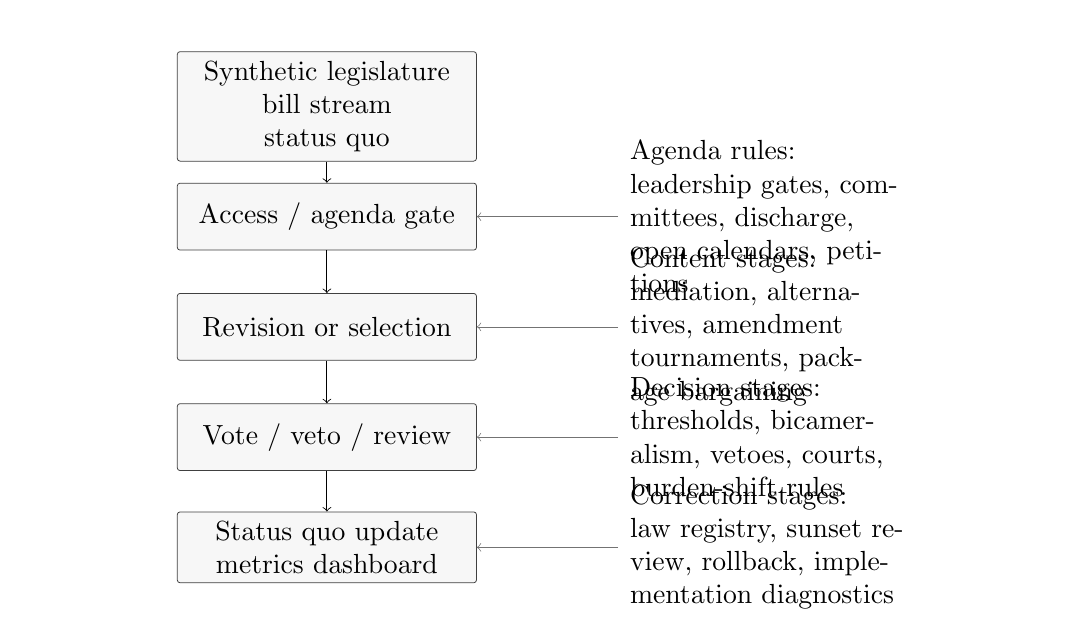
\begin{tikzpicture}[x=1mm,y=1mm]
\path[use as bounding box] (0,0) rectangle (130,74);
\tikzstyle{stage}=[draw=black!75, rounded corners=1pt, line width=0.28pt, align=center, minimum width=38mm, minimum height=8.5mm, fill=black!3]
\tikzstyle{side}=[align=left, text width=35mm]

\node[stage] (world) at (38,64) {Synthetic legislature\\bill stream\\status quo};
\node[stage] (access) at (38,50) {Access / agenda gate};
\node[stage] (revision) at (38,36) {Revision or selection};
\node[stage] (vote) at (38,22) {Vote / veto / review};
\node[stage] (metrics) at (38,8) {Status quo update\\metrics dashboard};

\draw[->, line width=0.3pt] (world) -- (access);
\draw[->, line width=0.3pt] (access) -- (revision);
\draw[->, line width=0.3pt] (revision) -- (vote);
\draw[->, line width=0.3pt] (vote) -- (metrics);

\node[side] at (94,50) {Agenda rules:\\leadership gates, committees, discharge, open calendars, petitions};
\draw[->, black!55, line width=0.25pt] (75,50) -- (access.east);

\node[side] at (94,36) {Content stages:\\mediation, alternatives, amendment tournaments, package bargaining};
\draw[->, black!55, line width=0.25pt] (75,36) -- (revision.east);

\node[side] at (94,22) {Decision stages:\\thresholds, bicameralism, vetoes, courts, burden-shift rules};
\draw[->, black!55, line width=0.25pt] (75,22) -- (vote.east);

\node[side] at (94,8) {Correction stages:\\law registry, sunset review, rollback, implementation diagnostics};
\draw[->, black!55, line width=0.25pt] (75,8) -- (metrics.east);
\end{tikzpicture}
\endgroup


  \caption{Modular simulation pipeline. Each institutional bundle intervenes at one or more stages while generated legislatures, bill streams, and status-quo-relative voting remain shared across comparisons.}
  \label{fig:simulation-pipeline}
  \Description{Pipeline diagram showing synthetic world generation, institutional routing, content transformation, collective decision, correction, and diagnostic dashboard output.}
\end{figure}

\section{Metrics and Campaign}

The simulator reports a dashboard rather than a single welfare score. Table~\ref{tab:metric-groups} defines the metrics used in the main paper; secondary diagnostics remain in generated reports and appendix tables.

\begin{table}
  \caption{Main metrics and interpretation.}
  \label{tab:metric-groups}
  \Description{A compact glossary table defining the main metrics, direction of interpretation, and caveats.}
  \scriptsize
  \setlength{\tabcolsep}{2.4pt}
  \resizebox{\linewidth}{!}{%
  \begin{tabular}{llll}
    \toprule
    Metric & Direction & Definition & Caveat \\
    \midrule
    Productivity & \(\uparrow\) & Share of submitted bills enacted. & Can reward bad throughput. \\
    Yield & \(\uparrow\) & Generated public benefit per submitted proposal. & Synthetic and generator-dependent. \\
    Revision moderation & \(\uparrow\) & Score combining moderation, legitimacy, and incrementalism. & Not a neutral welfare measure. \\
    Public support & \(\uparrow\) & Enacted-bill support composite from generated support signals. & Not observed public opinion. \\
    Low-support enactment & \(\downarrow\) & Enacted bills below 50\% generated support. & Depends on synthetic support threshold. \\
    Risk control & \(\uparrow\) & Inverse composite of harm, capture, low support, proposer gain, and policy shock. & Composite score. \\
    Admin feasibility & \(\uparrow\) & \(1-\) procedural-load index from attention, review, challenge, amendment, and selection costs. & Indirect cost proxy. \\
    \bottomrule
  \end{tabular}
  }
\end{table}

Yield prevents a system that blocks nearly all proposals from looking equivalent to one that produces generated public value. Risk control averages inverse low-support passage, minority harm, lobbying capture, public-preference distortion, concentrated-harm passage, proposer gain, and policy shock terms; administrative feasibility is \(1-\) the procedural-load index.

As one sensitivity check, the paper reports a revision-moderation-weighted value profile combining revision moderation, productivity, risk control, administrative feasibility, and public support. The main interpretation relies on metric-level tradeoffs rather than this scalar score.

All main results come from one reported comparison campaign. It combines broad assumptions, adversarial generator cases, weighted party-system cases, and a stylized rising-contention timeline in one CSV. The canonical run uses 120 generated worlds per case, 101 legislators, 60 bills per run, and seed 20260428. Cases vary polarization, party loyalty, revision-moderation culture, lobbying, constituency pressure, party count, proposal pressure, capture pressure, and anti-lobbying reform demand. The adversarial bill-stream cases stress extremity, capture, delayed benefits, concentrated harm, and backlash dynamics.

Scenario selection follows a fixed coverage rule: include the stylized U.S.-like benchmark, simple majority, committee regular order, discharge petition, open floor calendar, a combined content-selection family, anti-capture access, harm-weighted majority, one burden-shifting stress case, one burden-shifting mediation case, and a portfolio hybrid. The appendix reports the broader scenario catalog and fixed-rule family champions.

% Auto-generated by paper/scripts/generate_figures.py
\begin{table*}
  \caption{Mechanism families used in the main comparison. Labels match the Results figures; the appendix reports the broader implemented catalog.}
  \label{tab:design-space-coverage}
  \Description{A compact generated table showing the main mechanisms represented in the reported comparison, their labels, mechanism themes, and primary stress risks.}
  \small
  \begin{tabular}{@{}llll@{}}
    \toprule
    Family & Labels & Mechanism theme & Primary stress risk \\
    \midrule
    Conventional benchmark & CUR & House/Senate/veto gate & Bottlenecks \\
    Simple majority & SM & Affirmative threshold & Low screening \\
    Committee regular order & COMM & Committee-first gate & Burial/capture \\
    Discharge petition & DIS & Committee bypass & Bypass pressure \\
    Open floor calendar & OPEN & Default-open agenda & Floor overload \\
    Content selection & SEL & Alternatives/tournament & Clones/agenda manipulation \\
    Anti-capture access & ACG & Pre-floor capture screen & Gate bias \\
    Harm-weighted majority & HARM & Affected-group threshold & Holdouts \\
    Burden-shifting stress & DP & Pass unless blocked & False silence \\
    Burden shift + mediation & DPM & Mediation plus challenge & Cost/weak consent \\
    Portfolio hybrid & PORT & Combined safeguards & Complexity \\
    \bottomrule
  \end{tabular}
\end{table*}


The chamber-structure supplement tests representation architecture, committee power, eligibility filters, and ex ante review. It is separate because it asks how those structures shift the same productivity/revision-moderation tradeoff.

Empirical boundary checks are artifact screens, not calibration in the statistical sense. \texttt{make calibrate} compares conventional baselines with broad benchmark ranges derived from Voteview, Congress.gov, govinfo, Comparative Agendas Project, lobbying-disclosure and OpenFEC records, Center for Effective Lawmaking measures, SCDB merits cases, Federal Register final-rule records, Congress.gov public-law text flags, and institutional indicators \citep{Voteview2021,CongressGovData,GovinfoBillStatus2020,ComparativeAgendasProject,SenateLDA,OpenFECData,VoldenWiseman2014,VDemDataset}. Separate held-out and flow checks use documented empirical comparison samples: a 180-row Congress.gov bill-progression extract with a bounded govinfo BILLSTATUS cross-check over the same bill universe, a bounded sponsor aggregate with sponsor-bill metadata matches by Bioguide ID, a Voteview extract carrying bounded member metadata and bill-number linkage, a Senate LDA lobbying-disclosure extract with bounded issue-policy context, policy-area bill/action context, exact bill-identifier action metadata context, and bounded stored activity-text support/position signal review, a bounded OpenFEC campaign-finance extract plus FEC recipient metadata, broad transaction-label issue context, matched-candidate Voteview member context, House-candidate district context for small subsets, public FEC/OpenFEC target-scope review for queued campaign-finance rows, and cached committee/floor bill-action context for queued finance/lobbying rows, a bounded Cumulative CES district-opinion aggregate \citep{CumulativeCES2025} plus Congress.gov sponsor-district bill metadata, bounded bill policy-area context, a 22-bill public-opinion readiness queue with 0 issue-specific support rows and 0 affected-group support/harm rows, 22 source-acquisition packets with no acquired external bill-topic dataset, official Census TIGERweb population/housing denominators, and official ACS 2017--2021 broad district context, a bounded QoG/OWID/V-Dem comparative-institution profile with simulator scenario-family metadata anchors \citep{QoGDataFinder2026,BormannGolder2022,HeniszPOLCON2017,OWIDVDEMJudicial2026,OWIDVDEMLegislative2026}, SCDB merits review with bounded U.S.C.-section authority-overlap metadata, Federal Register final-rule effective dates, document/docket metadata, bounded public-law authority-search metadata, and bounded proposed-history/comment-portal/timing metadata, Congress.gov public-law revision text and bill-action metadata, and Congress.gov-derived topic and committee summaries. These support nine narrow held-out source-family checks covering bill attrition and floor load, roll-call coalition size, sponsor concentration, campaign-finance concentration and outside-spending share, district public-will proxies, SCDB merits invalidation, final-rule effective-delay, public-law revision text flags, and comparative bicameral context. The govinfo layer is an independent metadata cross-check for the bounded bill sample, while sponsor-bill metadata, district public-opinion policy-area context, district denominator and broad ACS context, comparative scenario-family metadata anchors, LDA issue-policy context, policy-area bill context, exact bill-identifier action context, stored LDA activity-text signals, FEC issue-sector and target-scope context, cached committee/floor bill-action context, Federal Register authority text, Federal Register proposed-history/comment-portal/timing metadata, SCDB U.S.C.-section overlap metadata, topic-throughput, and committee summaries remain flow or calibration proxy evidence. The generated linkage audit reports all thirteen source families as linked, metadata-linked, or partially linked, mostly through topic, policy-area, govinfo BILLSTATUS metadata, bounded sponsor-bill metadata, bounded comparative scenario-family metadata, Voteview member metadata and bounded bill-number linkage, LDA issue-taxonomy, policy-area bill context, exact bill-identifier action context, and stored activity-text signals, FEC recipient metadata, bounded FEC issue-sector, candidate-member, candidate-district, public target-scope context, and cached committee/floor bill-action context, Congress.gov sponsor-district metadata plus bill policy-area context and district context layers, SCDB/Federal Register U.S.C.-section overlap metadata, Federal Register document metadata and authority-text matches, or Congress.gov bill/action metadata joins. None of these checks is model validation.

% Auto-generated by scripts/reporting/write_paper_diagnostics.py
\begin{table}
  \caption{Selected empirical flow smoke tests. Raw inputs do not validate the synthetic welfare, revision moderation, harm, capture, or public-support metrics.}
  \label{tab:empirical-bridge}
  \Description{A generated table mapping empirical comparison signals to optional raw inputs and simulator proxies.}
  \scriptsize
  \setlength{\tabcolsep}{2.6pt}
  \resizebox{\linewidth}{!}{%
  \begin{tabular}{llll}
    \toprule
    Signal & Raw & Simulator proxy & Does not validate \\
    \midrule
    Bill attrition & enactmentRate=0.024 & current-congress-workflow/productivity & public benefit or law quality \\
    Floor consideration & floorLoad=0.067 & current-congress-workflow/floor & agenda fairness or policy merit \\
    Committee advancement from bill actions & committeeAdvanceRate=0.100 & current-congress-workflow/committeeAdvanceRate & committee expertise or capture \\
    Committee reporting from bill actions & committeeReportRate=0.064 & --- & committee expertise or capture \\
    Roll-call coalition size & coalitionSize=0.604 & current-system/averageEnactedSupport & public opinion \\
    Sponsor proposal concentration & sponsorIntroductionGini=0.389 & current-system/proposerAccessGini & capture or representational equity \\
    \bottomrule
  \end{tabular}
  }
\end{table}


\section{Results}

The selected mechanism-family comparison shows three patterns. First, throughput and support/risk diagnostics separate: mechanisms that enact more proposals can also enact more low-public-support proposals. Second, content-selection stages change the collective intelligence process by altering which alternatives enter final aggregation, not merely by changing the final yes/no threshold. Because pairwise alternatives and amendment tournaments produce nearly identical aggregate profiles in this campaign, the main text reports them as a single content-selection family. Third, portfolio safeguards reduce several risk diagnostics but increase procedural load. The stylized U.S.-like benchmark has low productivity but stronger revision moderation, risk, and support diagnostics than its directional profile suggests.

The empirical boundary checks are narrow screens for observable legislative-flow and roll-call proxies. They do not validate generated public benefit, revision moderation, harm, capture, representation, or public-support diagnostics.

The main robustness table reports numeric generator-sensitivity, vote-kernel-ablation, and seed-stability checks. Detailed Pareto checks, ablation deltas, manipulation-stress losses, and separate PAIR/AMT rows appear in the appendix. The generator-sensitivity rows and fairness controls show that the framework can expose dependence on generator assumptions, but they do not remove that dependence. These results are mechanism-behavior hypotheses under the implemented generator, not general rankings of legislative institutions.

The chamber-structure supplement is reported in the appendix. It asks a separate question about representation architecture and review design, so it is not part of the ACM paper's central evidence chain.

\begin{figure}[!htbp]
  \centering
  \begin{minipage}[t]{0.49\textwidth}
    \centering
    \resizebox{\linewidth}{!}{% Auto-generated by paper/scripts/generate_figures.py
\begingroup
\setlength{\unitlength}{1mm}
\begin{picture}(122,82)
\footnotesize
\put(16.0,13.0){\color{black!15}\line(0,1){58.0}}
\put(16.0,13.0){\color{black!15}\line(1,0){96.0}}
\put(16.0,9.9){\makebox(0,0){0}}
\put(12.8,13.0){\makebox(0,0)[r]{0}}
\put(40.0,13.0){\color{black!15}\line(0,1){58.0}}
\put(16.0,27.5){\color{black!15}\line(1,0){96.0}}
\put(40.0,9.9){\makebox(0,0){0.25}}
\put(12.8,27.5){\makebox(0,0)[r]{0.25}}
\put(64.0,13.0){\color{black!15}\line(0,1){58.0}}
\put(16.0,42.0){\color{black!15}\line(1,0){96.0}}
\put(64.0,9.9){\makebox(0,0){0.5}}
\put(12.8,42.0){\makebox(0,0)[r]{0.5}}
\put(88.0,13.0){\color{black!15}\line(0,1){58.0}}
\put(16.0,56.5){\color{black!15}\line(1,0){96.0}}
\put(88.0,9.9){\makebox(0,0){0.75}}
\put(12.8,56.5){\makebox(0,0)[r]{0.75}}
\put(112.0,13.0){\color{black!15}\line(0,1){58.0}}
\put(16.0,71.0){\color{black!15}\line(1,0){96.0}}
\put(112.0,9.9){\makebox(0,0){1}}
\put(12.8,71.0){\makebox(0,0)[r]{1}}
\put(16.0,13.0){\line(1,0){96.0}}
\put(16.0,13.0){\line(0,1){58.0}}
\put(112.0,13.0){\line(0,1){58.0}}
\put(16.0,71.0){\line(1,0){96.0}}
\put(21.0,67.0){\makebox(0,0){\color{red}\rule{2.1mm}{2.1mm}}}
\linethickness{0.10mm}
{\color{red!55}\qbezier[8](21.0,67.0)(22.3,64.1)(23.6,61.2)}
\linethickness{0.25mm}
% point-label label=1* pointX=21.0 pointY=67.0 labelX=24.8 labelY=61.2 anchor=l leader=1
\put(24.8,61.2){\makebox(0,0)[l]{\color{red}1*}}
\put(47.3,62.2){\makebox(0,0){\color{black}\rule{1.7mm}{1.7mm}}}
\linethickness{0.10mm}
{\color{black!35}\qbezier[8](47.3,62.2)(48.6,64.9)(49.9,67.5)}
\linethickness{0.25mm}
% point-label label=2 pointX=47.3 pointY=62.2 labelX=51.1 labelY=67.5 anchor=l leader=1
\put(51.1,67.5){\makebox(0,0)[l]{\color{black}2}}
\put(36.6,64.6){\makebox(0,0){\color{black}\rule{1.7mm}{1.7mm}}}
\linethickness{0.10mm}
{\color{black!35}\qbezier[8](36.6,64.6)(37.9,61.7)(39.2,58.8)}
\linethickness{0.25mm}
% point-label label=3 pointX=36.6 pointY=64.6 labelX=40.4 labelY=58.8 anchor=l leader=1
\put(40.4,58.8){\makebox(0,0)[l]{\color{black}3}}
\put(29.9,66.6){\makebox(0,0){\color{black}\rule{1.7mm}{1.7mm}}}
\linethickness{0.10mm}
{\color{black!35}\qbezier[8](29.9,66.6)(26.9,63.1)(23.9,59.6)}
\linethickness{0.25mm}
% point-label label=4 pointX=29.9 pointY=66.6 labelX=22.7 labelY=59.6 anchor=r leader=1
\put(22.7,59.6){\makebox(0,0)[r]{\color{black}4}}
\put(50.6,61.7){\makebox(0,0){\color{black}\rule{1.7mm}{1.7mm}}}
\linethickness{0.10mm}
{\color{black!35}\qbezier[8](50.6,61.7)(51.2,57.8)(51.8,53.9)}
\linethickness{0.25mm}
% point-label label=5 pointX=50.6 pointY=61.7 labelX=50.6 labelY=53.9 anchor=c leader=1
\put(50.6,53.9){\makebox(0,0)[c]{\color{black}5}}
\put(69.2,67.3){\makebox(0,0){\color{black}\rule{1.7mm}{1.7mm}}}
\linethickness{0.10mm}
{\color{black!35}\qbezier[8](69.2,67.3)(70.5,67.4)(71.8,67.5)}
\linethickness{0.25mm}
% point-label label=6 pointX=69.2 pointY=67.3 labelX=73.0 labelY=67.5 anchor=l leader=1
\put(73.0,67.5){\makebox(0,0)[l]{\color{black}6}}
\put(42.1,64.1){\makebox(0,0){\color{black}\rule{1.7mm}{1.7mm}}}
\linethickness{0.10mm}
{\color{black!35}\qbezier[8](42.1,64.1)(47.4,62.2)(52.6,60.3)}
\linethickness{0.25mm}
% point-label label=7 pointX=42.1 pointY=64.1 labelX=53.8 labelY=60.3 anchor=l leader=1
\put(53.8,60.3){\makebox(0,0)[l]{\color{black}7}}
\put(42.7,63.6){\makebox(0,0){\color{black}\rule{1.7mm}{1.7mm}}}
\linethickness{0.10mm}
{\color{black!35}\qbezier[8](42.7,63.6)(41.4,60.7)(40.1,57.8)}
\linethickness{0.25mm}
% point-label label=8 pointX=42.7 pointY=63.6 labelX=38.9 labelY=57.8 anchor=r leader=1
\put(38.9,57.8){\makebox(0,0)[r]{\color{black}8}}
\put(99.8,49.5){\makebox(0,0){\color{black}\rule{1.7mm}{1.7mm}}}
\linethickness{0.10mm}
{\color{black!35}\qbezier[8](99.8,49.5)(101.1,52.4)(102.4,55.3)}
\linethickness{0.25mm}
% point-label label=9 pointX=99.8 pointY=49.5 labelX=103.6 labelY=55.3 anchor=l leader=1
\put(103.6,55.3){\makebox(0,0)[l]{\color{black}9}}
\put(93.4,55.2){\makebox(0,0){\color{black}\rule{1.7mm}{1.7mm}}}
\linethickness{0.10mm}
{\color{black!35}\qbezier[8](93.4,55.2)(94.7,58.1)(96.0,61.0)}
\linethickness{0.25mm}
% point-label label=10 pointX=93.4 pointY=55.2 labelX=97.2 labelY=61.0 anchor=l leader=1
\put(97.2,61.0){\makebox(0,0)[l]{\color{black}10}}
\put(67.1,67.0){\makebox(0,0){\color{black}\rule{1.7mm}{1.7mm}}}
\linethickness{0.10mm}
{\color{black!35}\qbezier[8](67.1,67.0)(65.8,67.3)(64.5,67.5)}
\linethickness{0.25mm}
% point-label label=11 pointX=67.1 pointY=67.0 labelX=63.3 labelY=67.5 anchor=r leader=1
\put(63.3,67.5){\makebox(0,0)[r]{\color{black}11}}
\put(64.0,76.8){\makebox(0,0){Risk control (higher is better)}}
\put(64.0,2.0){\makebox(0,0){Productivity (share enacted; higher is better)}}
\end{picture}
\endgroup
}
    \vspace{-0.75\baselineskip}
    \centerline{\small (a) Risk control}
  \end{minipage}\hfill
  \begin{minipage}[t]{0.49\textwidth}
    \centering
    \resizebox{\linewidth}{!}{% Auto-generated by paper/scripts/generate_figures.py
\begingroup
\setlength{\unitlength}{1mm}
\begin{picture}(122,82)
\footnotesize
\put(16.0,13.0){\color{black!15}\line(0,1){58.0}}
\put(16.0,13.0){\color{black!15}\line(1,0){96.0}}
\put(16.0,9.9){\makebox(0,0){0}}
\put(12.8,13.0){\makebox(0,0)[r]{0}}
\put(40.0,13.0){\color{black!15}\line(0,1){58.0}}
\put(16.0,27.5){\color{black!15}\line(1,0){96.0}}
\put(40.0,9.9){\makebox(0,0){0.25}}
\put(12.8,27.5){\makebox(0,0)[r]{0.25}}
\put(64.0,13.0){\color{black!15}\line(0,1){58.0}}
\put(16.0,42.0){\color{black!15}\line(1,0){96.0}}
\put(64.0,9.9){\makebox(0,0){0.5}}
\put(12.8,42.0){\makebox(0,0)[r]{0.5}}
\put(88.0,13.0){\color{black!15}\line(0,1){58.0}}
\put(16.0,56.5){\color{black!15}\line(1,0){96.0}}
\put(88.0,9.9){\makebox(0,0){0.75}}
\put(12.8,56.5){\makebox(0,0)[r]{0.75}}
\put(112.0,13.0){\color{black!15}\line(0,1){58.0}}
\put(16.0,71.0){\color{black!15}\line(1,0){96.0}}
\put(112.0,9.9){\makebox(0,0){1}}
\put(12.8,71.0){\makebox(0,0)[r]{1}}
\put(16.0,13.0){\line(1,0){96.0}}
\put(16.0,13.0){\line(0,1){58.0}}
\put(112.0,13.0){\line(0,1){58.0}}
\put(16.0,71.0){\line(1,0){96.0}}
\put(21.2,35.0){\makebox(0,0){\color{black}\rule{2.5mm}{2.5mm}}}
\linethickness{0.10mm}
{\color{black!35}\qbezier[8](21.2,35.0)(22.5,37.9)(23.8,40.8)}
\linethickness{0.25mm}
% point-label label=CUR* pointX=21.2 pointY=35.0 labelX=25.0 labelY=40.8 anchor=l leader=1
\put(25.0,40.8){\makebox(0,0)[l]{\color{black}CUR*}}
\put(42.6,26.6){\makebox(0,0){\color{black}\rule{1.8mm}{1.8mm}}}
\linethickness{0.10mm}
{\color{black!35}\qbezier[8](42.6,26.6)(43.9,29.5)(45.2,32.4)}
\linethickness{0.25mm}
% point-label label=SM pointX=42.6 pointY=26.6 labelX=46.4 labelY=32.4 anchor=l leader=1
\put(46.4,32.4){\makebox(0,0)[l]{\color{black}SM}}
\put(32.3,29.7){\makebox(0,0){\color{black}\rule{1.8mm}{1.8mm}}}
\linethickness{0.10mm}
{\color{black!35}\qbezier[8](32.3,29.7)(31.0,26.8)(29.7,23.9)}
\linethickness{0.25mm}
% point-label label=COMM pointX=32.3 pointY=29.7 labelX=28.5 labelY=23.9 anchor=r leader=1
\put(28.5,23.9){\makebox(0,0)[r]{\color{black}COMM}}
\put(31.5,30.9){\makebox(0,0){\color{black}\rule{1.8mm}{1.8mm}}}
\linethickness{0.10mm}
{\color{black!35}\qbezier[8](31.5,30.9)(32.8,33.8)(34.1,36.7)}
\linethickness{0.25mm}
% point-label label=DIS pointX=31.5 pointY=30.9 labelX=35.3 labelY=36.7 anchor=l leader=1
\put(35.3,36.7){\makebox(0,0)[l]{\color{black}DIS}}
\put(46.7,26.8){\makebox(0,0){\color{black}\rule{1.8mm}{1.8mm}}}
\linethickness{0.10mm}
{\color{black!35}\qbezier[8](46.7,26.8)(49.4,27.2)(52.1,27.7)}
\linethickness{0.25mm}
% point-label label=OPEN pointX=46.7 pointY=26.8 labelX=53.3 labelY=27.7 anchor=l leader=1
\put(53.3,27.7){\makebox(0,0)[l]{\color{black}OPEN}}
\put(68.1,42.9){\makebox(0,0){\color{black}\rule{1.8mm}{1.8mm}}}
\linethickness{0.10mm}
{\color{black!35}\qbezier[8](68.1,42.9)(69.4,45.8)(70.7,48.7)}
\linethickness{0.25mm}
% point-label label=SEL pointX=68.1 pointY=42.9 labelX=71.9 labelY=48.7 anchor=l leader=1
\put(71.9,48.7){\makebox(0,0)[l]{\color{black}SEL}}
\put(42.5,26.7){\makebox(0,0){\color{black}\rule{1.8mm}{1.8mm}}}
\linethickness{0.10mm}
{\color{black!35}\qbezier[8](42.5,26.7)(43.8,23.8)(45.1,20.9)}
\linethickness{0.25mm}
% point-label label=ACG pointX=42.5 pointY=26.7 labelX=46.3 labelY=20.9 anchor=l leader=1
\put(46.3,20.9){\makebox(0,0)[l]{\color{black}ACG}}
\put(41.4,26.8){\makebox(0,0){\color{black}\rule{1.8mm}{1.8mm}}}
\linethickness{0.10mm}
{\color{black!35}\qbezier[8](41.4,26.8)(40.1,23.9)(38.8,21.0)}
\linethickness{0.25mm}
% point-label label=HARM pointX=41.4 pointY=26.8 labelX=37.6 labelY=21.0 anchor=r leader=1
\put(37.6,21.0){\makebox(0,0)[r]{\color{black}HARM}}
\put(96.1,19.5){\makebox(0,0){\color{black}\rule{1.8mm}{1.8mm}}}
\linethickness{0.10mm}
{\color{black!35}\qbezier[8](96.1,19.5)(97.4,22.4)(98.7,25.3)}
\linethickness{0.25mm}
% point-label label=DP pointX=96.1 pointY=19.5 labelX=99.9 labelY=25.3 anchor=l leader=1
\put(99.9,25.3){\makebox(0,0)[l]{\color{black}DP}}
\put(82.1,26.1){\makebox(0,0){\color{black}\rule{1.8mm}{1.8mm}}}
\linethickness{0.10mm}
{\color{black!35}\qbezier[8](82.1,26.1)(83.4,29.0)(84.7,31.9)}
\linethickness{0.25mm}
% point-label label=DPM pointX=82.1 pointY=26.1 labelX=85.9 labelY=31.9 anchor=l leader=1
\put(85.9,31.9){\makebox(0,0)[l]{\color{black}DPM}}
\put(66.6,36.7){\makebox(0,0){\color{black}\rule{1.8mm}{1.8mm}}}
\linethickness{0.10mm}
{\color{black!35}\qbezier[8](66.6,36.7)(65.3,39.6)(64.0,42.5)}
\linethickness{0.25mm}
% point-label label=PORT pointX=66.6 pointY=36.7 labelX=62.8 labelY=42.5 anchor=r leader=1
\put(62.8,42.5){\makebox(0,0)[r]{\color{black}PORT}}
\put(64.0,76.8){\makebox(0,0){Revision moderation (higher is better)}}
\put(64.0,2.0){\makebox(0,0){Productivity (share enacted; higher is better)}}
\end{picture}
\endgroup
}
    \vspace{-0.75\baselineskip}
    \centerline{\small (b) Revision moderation}
  \end{minipage}
  \caption{Productivity tradeoff views for the representative systems. Panel (a) plots risk control across the main broad/adversarial campaign averages, with thin five-seed uncertainty bars where visible; panel (b) plots revision moderation under weighted party-system sensitivity cases. Higher is better on both y-axes. Labels are the mechanism-family labels from Table~\ref{tab:design-space-coverage}. The asterisk and larger square mark the stylized U.S.-like benchmark.}
  \label{fig:productivity-tradeoffs}
  \Description{Two side-by-side scatter plots with the same productivity axis: one compares productivity against risk control, and the other compares productivity against revision moderation.}
\end{figure}

The burden-shifting stress cases illustrate the same separation. Open burden-shifting passage has high productivity but weak revision-moderation and support diagnostics, while mediation improves some content metrics at additional procedural cost. These results are best read as failure-mode probes rather than as a central reform comparison.

Manipulation-stress cases use bounded adversaries rather than fully co-evolving strategic parties. The adversary can choose clone or decoy proposals, noisier citizen-panel information, loose harm claims, astroturf objection pressure, proposal flooding, or anti-lobbying backlash under fixed information and budget assumptions. Stress objectives are enactment of low-support bills, blockage of high-benefit bills, or administrative overload. Appendix tables report paired losses, while adaptive worst-case search remains future work.

The portfolio variants illustrate the tradeoff between combining safeguards and increasing administrative load. They improve several risk diagnostics but do not dominate simpler alternative-selection mechanisms.

% Auto-generated by paper/scripts/generate_figures.py
\begingroup
\setlength{\unitlength}{1mm}
\begin{picture}(128,88)
\scriptsize
\put(34.1,84.5){\makebox(0,0){\textbf{Prod.}}}
\put(26.0,81.0){\color{black!20}\line(1,0){16.2}}
\put(50.3,84.5){\makebox(0,0){\textbf{Comp.}}}
\put(42.2,81.0){\color{black!20}\line(1,0){16.2}}
\put(66.5,84.5){\makebox(0,0){\textbf{Public}}}
\put(58.4,81.0){\color{black!20}\line(1,0){16.2}}
\put(82.7,84.5){\makebox(0,0){\textbf{Risk}}}
\put(74.6,81.0){\color{black!20}\line(1,0){16.2}}
\put(98.9,84.5){\makebox(0,0){\textbf{Admin}}}
\put(90.8,81.0){\color{black!20}\line(1,0){16.2}}
\put(115.1,84.5){\makebox(0,0){\textbf{Sens.}}}
\put(107.0,81.0){\color{black!20}\line(1,0){16.2}}
\put(20.0,76.0){\makebox(0,0)[r]{\color{black}\textbf{CUR*}}}
\put(26.0,75.5){\color{black!7}\rule{15.6mm}{2.4mm}}
\put(33.8,76.7){\makebox(0,0){\color{black}\textbf{0.05}}}
\put(42.2,75.5){\color{black!16}\rule{15.6mm}{2.4mm}}
\put(50.0,76.7){\makebox(0,0){\color{black}\textbf{0.36}}}
\put(58.4,75.5){\color{black!30}\rule{15.6mm}{2.4mm}}
\put(66.2,76.7){\makebox(0,0){\color{black}\textbf{0.77}}}
\put(74.6,75.5){\color{black!35}\rule{15.6mm}{2.4mm}}
\put(82.4,76.7){\makebox(0,0){\color{black}\textbf{0.93}}}
\put(90.8,75.5){\color{black!37}\rule{15.6mm}{2.4mm}}
\put(98.6,76.7){\makebox(0,0){\color{black}\textbf{0.98}}}
\put(107.0,75.5){\color{black!23}\rule{15.6mm}{2.4mm}}
\put(114.8,76.7){\makebox(0,0){\color{black}\textbf{0.57}}}
\put(20.0,73.0){\makebox(0,0)[r]{\color{black}SM}}
\put(26.0,72.5){\color{black!15}\rule{15.6mm}{2.4mm}}
\put(33.8,73.7){\makebox(0,0){\color{black}0.33}}
\put(42.2,72.5){\color{black!13}\rule{15.6mm}{2.4mm}}
\put(50.0,73.7){\makebox(0,0){\color{black}0.24}}
\put(58.4,72.5){\color{black!27}\rule{15.6mm}{2.4mm}}
\put(66.2,73.7){\makebox(0,0){\color{black}0.68}}
\put(74.6,72.5){\color{black!32}\rule{15.6mm}{2.4mm}}
\put(82.4,73.7){\makebox(0,0){\color{black}0.85}}
\put(90.8,72.5){\color{black!35}\rule{15.6mm}{2.4mm}}
\put(98.6,73.7){\makebox(0,0){\color{black}0.93}}
\put(107.0,72.5){\color{black!23}\rule{15.6mm}{2.4mm}}
\put(114.8,73.7){\makebox(0,0){\color{black}0.55}}
\put(20.0,70.0){\makebox(0,0)[r]{\color{black}COMM}}
\put(26.0,69.6){\color{black!12}\rule{15.6mm}{2.4mm}}
\put(33.8,70.8){\makebox(0,0){\color{black}0.22}}
\put(42.2,69.6){\color{black!14}\rule{15.6mm}{2.4mm}}
\put(50.0,70.8){\makebox(0,0){\color{black}0.28}}
\put(58.4,69.6){\color{black!28}\rule{15.6mm}{2.4mm}}
\put(66.2,70.8){\makebox(0,0){\color{black}0.73}}
\put(74.6,69.6){\color{black!33}\rule{15.6mm}{2.4mm}}
\put(82.4,70.8){\makebox(0,0){\color{black}0.89}}
\put(90.8,69.6){\color{black!36}\rule{15.6mm}{2.4mm}}
\put(98.6,70.8){\makebox(0,0){\color{black}0.97}}
\put(107.0,69.6){\color{black!23}\rule{15.6mm}{2.4mm}}
\put(114.8,70.8){\makebox(0,0){\color{black}0.56}}
\put(20.0,67.1){\makebox(0,0)[r]{\color{black}DIS}}
\put(26.0,66.7){\color{black!10}\rule{15.6mm}{2.4mm}}
\put(33.8,67.8){\makebox(0,0){\color{black}0.14}}
\put(42.2,66.7){\color{black!15}\rule{15.6mm}{2.4mm}}
\put(50.0,67.8){\makebox(0,0){\color{black}0.31}}
\put(58.4,66.7){\color{black!29}\rule{15.6mm}{2.4mm}}
\put(66.2,67.8){\makebox(0,0){\color{black}0.75}}
\put(74.6,66.7){\color{black!35}\rule{15.6mm}{2.4mm}}
\put(82.4,67.8){\makebox(0,0){\color{black}0.92}}
\put(90.8,66.7){\color{black!35}\rule{15.6mm}{2.4mm}}
\put(98.6,67.8){\makebox(0,0){\color{black}0.92}}
\put(107.0,66.7){\color{black!23}\rule{15.6mm}{2.4mm}}
\put(114.8,67.8){\makebox(0,0){\color{black}0.56}}
\put(20.0,64.2){\makebox(0,0)[r]{\color{black}OPEN}}
\put(26.0,63.7){\color{black!17}\rule{15.6mm}{2.4mm}}
\put(33.8,64.9){\makebox(0,0){\color{black}0.36}}
\put(42.2,63.7){\color{black!13}\rule{15.6mm}{2.4mm}}
\put(50.0,64.9){\makebox(0,0){\color{black}0.25}}
\put(58.4,63.7){\color{black!26}\rule{15.6mm}{2.4mm}}
\put(66.2,64.9){\makebox(0,0){\color{black}0.67}}
\put(74.6,63.7){\color{black!32}\rule{15.6mm}{2.4mm}}
\put(82.4,64.9){\makebox(0,0){\color{black}0.84}}
\put(90.8,63.7){\color{black!34}\rule{15.6mm}{2.4mm}}
\put(98.6,64.9){\makebox(0,0){\color{black}0.90}}
\put(107.0,63.7){\color{black!23}\rule{15.6mm}{2.4mm}}
\put(114.8,64.9){\makebox(0,0){\color{black}0.55}}
\put(20.0,61.2){\makebox(0,0)[r]{\color{black}SEL}}
\put(26.0,60.8){\color{black!23}\rule{15.6mm}{2.4mm}}
\put(33.8,61.9){\makebox(0,0){\color{black}0.55}}
\put(42.2,60.8){\color{black!21}\rule{15.6mm}{2.4mm}}
\put(50.0,61.9){\makebox(0,0){\color{black}0.50}}
\put(58.4,60.8){\color{black!30}\rule{15.6mm}{2.4mm}}
\put(66.2,61.9){\makebox(0,0){\color{black}0.79}}
\put(74.6,60.8){\color{black!35}\rule{15.6mm}{2.4mm}}
\put(82.4,61.9){\makebox(0,0){\color{black}0.94}}
\put(90.8,60.8){\color{black!28}\rule{15.6mm}{2.4mm}}
\put(98.6,61.9){\makebox(0,0){\color{black}0.71}}
\put(107.0,60.8){\color{black!27}\rule{15.6mm}{2.4mm}}
\put(114.8,61.9){\makebox(0,0){\color{black}0.67}}
\put(20.0,58.2){\makebox(0,0)[r]{\color{black}ACG}}
\put(26.0,57.8){\color{black!14}\rule{15.6mm}{2.4mm}}
\put(33.8,59.0){\makebox(0,0){\color{black}0.27}}
\put(42.2,57.8){\color{black!13}\rule{15.6mm}{2.4mm}}
\put(50.0,59.0){\makebox(0,0){\color{black}0.25}}
\put(58.4,57.8){\color{black!27}\rule{15.6mm}{2.4mm}}
\put(66.2,59.0){\makebox(0,0){\color{black}0.70}}
\put(74.6,57.8){\color{black!33}\rule{15.6mm}{2.4mm}}
\put(82.4,59.0){\makebox(0,0){\color{black}0.88}}
\put(90.8,57.8){\color{black!35}\rule{15.6mm}{2.4mm}}
\put(98.6,59.0){\makebox(0,0){\color{black}0.94}}
\put(107.0,57.8){\color{black!23}\rule{15.6mm}{2.4mm}}
\put(114.8,59.0){\makebox(0,0){\color{black}0.55}}
\put(20.0,55.3){\makebox(0,0)[r]{\color{black}HARM}}
\put(26.0,54.8){\color{black!14}\rule{15.6mm}{2.4mm}}
\put(33.8,56.0){\makebox(0,0){\color{black}0.28}}
\put(42.2,54.8){\color{black!13}\rule{15.6mm}{2.4mm}}
\put(50.0,56.0){\makebox(0,0){\color{black}0.26}}
\put(58.4,54.8){\color{black!27}\rule{15.6mm}{2.4mm}}
\put(66.2,56.0){\makebox(0,0){\color{black}0.69}}
\put(74.6,54.8){\color{black!33}\rule{15.6mm}{2.4mm}}
\put(82.4,56.0){\makebox(0,0){\color{black}0.87}}
\put(90.8,54.8){\color{black!35}\rule{15.6mm}{2.4mm}}
\put(98.6,56.0){\makebox(0,0){\color{black}0.93}}
\put(107.0,54.8){\color{black!23}\rule{15.6mm}{2.4mm}}
\put(114.8,56.0){\makebox(0,0){\color{black}0.55}}
\put(20.0,52.4){\makebox(0,0)[r]{\color{black}DP}}
\put(26.0,51.9){\color{black!33}\rule{15.6mm}{2.4mm}}
\put(33.8,53.1){\makebox(0,0){\color{black}0.87}}
\put(42.2,51.9){\color{black!9}\rule{15.6mm}{2.4mm}}
\put(50.0,53.1){\makebox(0,0){\color{black}0.14}}
\put(58.4,51.9){\color{black!23}\rule{15.6mm}{2.4mm}}
\put(66.2,53.1){\makebox(0,0){\color{black}0.57}}
\put(74.6,51.9){\color{black!25}\rule{15.6mm}{2.4mm}}
\put(82.4,53.1){\makebox(0,0){\color{black}0.63}}
\put(90.8,51.9){\color{black!35}\rule{15.6mm}{2.4mm}}
\put(98.6,53.1){\makebox(0,0){\color{black}0.93}}
\put(107.0,51.9){\color{black!23}\rule{15.6mm}{2.4mm}}
\put(114.8,53.1){\makebox(0,0){\color{black}0.57}}
\put(20.0,49.4){\makebox(0,0)[r]{\color{black}DPM}}
\put(26.0,49.0){\color{black!31}\rule{15.6mm}{2.4mm}}
\put(33.8,50.1){\makebox(0,0){\color{black}0.81}}
\put(42.2,49.0){\color{black!13}\rule{15.6mm}{2.4mm}}
\put(50.0,50.1){\makebox(0,0){\color{black}0.24}}
\put(58.4,49.0){\color{black!25}\rule{15.6mm}{2.4mm}}
\put(66.2,50.1){\makebox(0,0){\color{black}0.62}}
\put(74.6,49.0){\color{black!28}\rule{15.6mm}{2.4mm}}
\put(82.4,50.1){\makebox(0,0){\color{black}0.73}}
\put(90.8,49.0){\color{black!30}\rule{15.6mm}{2.4mm}}
\put(98.6,50.1){\makebox(0,0){\color{black}0.79}}
\put(107.0,49.0){\color{black!24}\rule{15.6mm}{2.4mm}}
\put(114.8,50.1){\makebox(0,0){\color{black}0.59}}
\put(20.0,46.5){\makebox(0,0)[r]{\color{black}PORT}}
\put(26.0,46.0){\color{black!22}\rule{15.6mm}{2.4mm}}
\put(33.8,47.2){\makebox(0,0){\color{black}0.53}}
\put(42.2,46.0){\color{black!19}\rule{15.6mm}{2.4mm}}
\put(50.0,47.2){\makebox(0,0){\color{black}0.43}}
\put(58.4,46.0){\color{black!29}\rule{15.6mm}{2.4mm}}
\put(66.2,47.2){\makebox(0,0){\color{black}0.76}}
\put(74.6,46.0){\color{black!35}\rule{15.6mm}{2.4mm}}
\put(82.4,47.2){\makebox(0,0){\color{black}0.93}}
\put(90.8,46.0){\color{black!29}\rule{15.6mm}{2.4mm}}
\put(98.6,47.2){\makebox(0,0){\color{black}0.76}}
\put(107.0,46.0){\color{black!26}\rule{15.6mm}{2.4mm}}
\put(114.8,47.2){\makebox(0,0){\color{black}0.65}}
\put(20.0,84.5){\makebox(0,0)[r]{\textbf{Label}}}
\put(74.6,1.4){\makebox(0,0){Rows grouped by mechanism family; values carry the comparison and shading is secondary.}}
\end{picture}
\endgroup


% Auto-generated by paper/scripts/generate_figures.py
\begin{table*}
  \caption{Main robustness checks with numeric evidence.}
  \label{tab:robustness-summary}
  \Description{A compact generated table reporting numeric robustness evidence for generator sensitivity, vote-kernel ablation, and seed stability.}
  \scriptsize
  \setlength{\tabcolsep}{2.2pt}
  \resizebox{\textwidth}{!}{%
  \begin{tabular}{lrrrrp{0.43\textwidth}}
    \toprule
    Check & SEL & PORT & DP/SM & Rank $\rho$ & Main implication \\
    \midrule
    High-benefit extreme & 0.69 & 0.72 & 0.57 & 0.95 & Moderation-friendly generator is relaxed by allowing high-distance bills to carry high generated value. \\
    Revision dilution & 0.67 & 0.71 & 0.67 & 0.78 & Moving toward the center can reduce generated public benefit. \\
    Lobby information & 0.74 & 0.71 & 0.28 & 0.70 & Organized lobbying can supply useful technical information rather than only capture pressure. \\
    Public-opinion error & 0.68 & 0.68 & 0.41 & 0.93 & Generated support and generated benefit are decoupled by noisy or biased support signals. \\
    Minority-rights harm & 0.66 & 0.64 & 0.19 & 0.57 & Majority-supported bills can impose concentrated rights-like harm. \\
    No support/revision vote & 0.57 & --- & SM 0.49 & --- & Vote-kernel ablation removes public-support and revision-moderation vote inputs while retaining them as diagnostics. \\
    Five-seed sweep & 0.699--0.701 & 0.700--0.701 & 0.733--0.734 & n=5 & Entries show directional-score min--max across independent base seeds; ranges are small relative to mechanism-family differences. \\
    \bottomrule
  \end{tabular}%
  }
  \par\smallskip\footnotesize \emph{Note:} SEL and PORT entries report the example profile except in the seed row, where they report directional-score min--max. DP/SM reports default-pass low-public-support enactment for generator checks, the no-signal simple-majority profile for the vote-kernel ablation, and default-pass seed range for the seed sweep. Rank $\rho$ is the Spearman correlation of displayed mechanism-family profile ranks against the main broad/adversarial average.
\end{table*}


The reported ordering should therefore be read as a hypothesis about mechanism behavior under the implemented generator, not as an institutional ranking.

\section{Limitations}

The model is stylized. It uses one primary policy dimension, generated legislators, generated support and benefit, simplified issue domains, and abstract lobbying units. The multidimensional package scenario is a cross-issue bargaining proxy, not a full two-dimensional ideal-point model; claims about alternatives, tournaments, revision moderation, and package bargaining are therefore intentionally narrow. Public-support diagnostics distinguish salience and costly affected-group pressure from cheap amplified volume, but they are still proxies. Because public benefit is internal to the generator, welfare comparisons are conditional on model assumptions. Systems that screen extreme, uncertain, or lobby-heavy bills may look better partly because the generator often encodes those features as lower expected public value. Adversarial cases partially relax this assumption, but welfare remains a synthetic signal.

The empirical layer screens conventional baselines against empirical ranges, and the held-out and flow smoke tests cover documented empirical inputs.
That is enough to make several agenda-access, legislative-flow, roll-call, campaign-finance, district-opinion, review, implementation-delay, revision-text, and comparative-profile proxies inspectable, but it is not enough for model validation or parameter fitting.
The linkage report currently documents topic-policy-area joins, committee-topic joins, a govinfo BILLSTATUS metadata cross-check for 180 of 180 cached bill-progression rows, bounded LDA issue-to-policy-area context for 144 of 146 cached lobbying rows, 308 issue-policy bill contexts across 144 unique cached bills and 3 unique enacted cached bills by shared policy area, 484 exact official LDA activity-text bill mention rows across 26 cached public-law bill IDs, cached Congress.gov bill/action metadata for those 26 exact-mentioned bills, stored LDA activity-text review that locates the bill reference in all 484 rows and classifies 46 support-only text-signal rows, 3 opposition-only text-signal rows, 2 mixed support/opposition rows, 104 position/activity rows, and 329 list/title-only rows, plus a disposition/target source-review queue prioritizing 156 rows for manual review, high-priority manual review for 4 rows, 102 medium-priority review packets representing the remaining 152 medium-priority rows, directional packet review for 28 support/opposition packets confirming 20 current-bill support packets and 1 current-bill opposition packet while downgrading 7 packets, and position/activity packet review for 74 packets representing 104 rows classifying 59 issue/provision activity packets, 5 monitoring/analysis packets, 7 all-provisions packets, 2 position-represented packets, and 1 current-bill opposition packet found in the position/activity queue, with no cached exact-match rows blocked by local truncation, an FEC recipient-metadata join for 192 of 194 campaign-finance rows, bounded OpenFEC transaction-label issue-topic context for 46 of 194 campaign-finance rows across 8 broad policy topics, matched-candidate Voteview member context for 30 campaign-finance transaction rows, bounded House-candidate district context for 23 campaign-finance transaction rows, bounded candidate-to-sponsored-bill context for 3 matched campaign-finance transaction rows across 9 cached bill IDs, sponsor-district public-law bill metadata for 63 of 1305 district-opinion row keys, bounded bill policy-area context for 66 sponsor-district public-law rows across 22 bills and 11 local policy areas, plus a bill-topic readiness queue covering those 22 bills with 0 issue-specific support rows, 0 affected-group support/harm rows, 22 source-acquisition packets across 11 policy areas with no acquired external bill-topic dataset, official Census TIGERweb population/housing denominators for 22 source packets across 21 sponsor districts, official ACS 2017--2021 broad district context for the same 22 source packets across 21 sponsor districts, and 22 survey-source crosswalk rows across 7 official source families with no acquired item IDs or estimates, SCDB/Federal Register U.S.C.-section overlaps for 26 of 9341 SCDB merits rows across 9 cached public-law rows and 12 normalized sections, Federal Register document/docket metadata for 495 of 500 implementation rows, Federal Register authority-text matches for 15 of 40 cached public-law rows across 51 rule documents, proposed-rule history matches for 23 of those 51 authority-matched final-rule rows across 36 proposed-rule links, proposed-rule Regulations.gov comment-portal metadata where available, 48 authority-matched final-rule rows with final effective dates, 23 proposed-to-final timing rows, and Congress.gov bill/action metadata for 40 of 120 public-law revision rows.
The bill-law spine attaches same-policy campaign-finance sponsor context to 17 public-law rows, same-policy LDA issue/bill context to 36 public-law rows, exact official LDA filing-text bill identifiers for 26 public-law rows, exact LDA bill/action metadata context for those 26 rows, and bounded stored LDA activity-text signals; these are context, identifier, text-signal, activity-text disposition, and metadata evidence, not bill-specific influence.
Separate govinfo, court-law, rulemaking-authority, rulemaking-history, bill-law, district-public-opinion policy-context, district-public-opinion bill-topic readiness, district-public-opinion source-packet, district-public-opinion Census denominator, district-public-opinion ACS context, district-public-opinion survey-source crosswalk, lobbying issue-linkage, lobbying bill-policy context, lobbying bill-mention review, lobbying bill-action context, lobbying bill-text review, lobbying bill-disposition review, lobbying manual-disposition review, lobbying medium-packet review, lobbying medium-directional packet review, lobbying medium-position/activity packet review, campaign-finance district-context, campaign-finance member-context, campaign-finance issue-context, campaign-finance sponsor-bill context, and bill-finance/lobbying committee-action context reports expose these bounded joins and the missing evidence that remains.
Bill-topic district opinion beyond sponsor-district policy-area context, the bill-topic readiness queue, source-acquisition packets, Census population/housing denominators, broad ACS district context, and survey-source crosswalk planning, bill-text-specific affected-population detail, affected-group representation, lobbying sponsor/member targeting and influence beyond exact filing-text bill identifiers, cached bill/action metadata context, and bounded stored text signals, bill-linked campaign finance beyond the current issue-sector/member/district/sponsored-bill and same-policy context, direct case-to-public-law review beyond U.S.C.-section overlap, emergency court review, fuller implementation feedback beyond document metadata, authority citations, proposed-rule/comment-portal metadata, and timing metadata, full statutory lineage beyond bill/action metadata, and observed cross-national institutional productivity or fit remain validation gaps; findings that depend on those components should be read as synthetic design hypotheses.
The Cumulative CES district aggregate is a direct survey proxy, not MRP, bill-topic support, or affected-group harm validation.
The committee and sponsor summaries are derived from sampled Congress.gov bill actions and are especially rough; the govinfo cache cross-checks the same bounded bill universe rather than replacing it with a full census.
The OpenFEC sample supports concentration, outside-spending summaries, public recipient metadata, bounded issue-sector context, bounded candidate-member context, bounded House-candidate district context, bounded candidate-to-sponsored-bill context, public target-scope review, and cached committee/floor bill-action flags for queued rows only, not causal influence, committee-action influence, legislative-outcome causality, or bill-level capture.
The LDA sample supports spending concentration, issue-taxonomy context, policy-area bill/action context, exact filing-text bill identifiers, exact bill/action metadata context, bounded stored activity-text support/position signals, a manual-review queue, a 4-row high-priority manual review slice, 102 medium-priority review packets, source-reviewed directional and position/activity packet dispositions, external current-bill mention-packet review, and cached committee/floor bill-action flags for a public-law subset only, not lobbying-contact confirmation, sponsor targeting beyond activity-text references, committee-action influence, roll-call influence, legislative-outcome causality, public benefit, or capture validation.
Congress.gov public-law revision rows support only amendment, reauthorization/extension, repeal, sunset/expiration text flags, bounded bill/action metadata, same-policy finance/lobbying context, exact LDA bill identifiers and bill/action context, authority-search metadata, proposed-history/comment-portal metadata, timing metadata, bounded court U.S.C.-section overlap metadata, and the derived spine inventory, not codified lineage, complete comments, implementation outcomes, bill-specific finance/lobbying influence, or direct court invalidation.
Fixture samples exercise adapter shapes but are not validation data.
Strategic behavior remains bounded: proposers and lobby groups adapt, and norm erosion can raise delay, but parties, committees, coalitions, courts, agencies, media, and elections do not yet co-evolve.
Chamber scenarios are sensitivity prototypes.
Citizen panels, initiatives, objection windows, tournaments, audits, challenge tokens, judicial review, and law-registry review are optimistic prototypes whose costs are represented only indirectly.
Package bargaining models side payments, delay, jurisdictional trades, and distributive load, not legal text or appropriations.

\section{Reproducibility}

The submitted manuscript is anonymized for double-blind review.
The artifact is a Java 21 project with Makefile entrypoints and vendored/generated CSV summaries for the paper workflow.
\texttt{make reproduce-paper-offline} is the no-network reproduction target; it regenerates the campaign, diagnostics, figures, PDFs, word-count check, anonymity scan, figure-label and table consistency checks, and PDF manifest from fixed seeds.
\texttt{make supplement-anonymous} builds the double-blind supplement.
Optional fixture samples can be refreshed with \texttt{make fetch-validation-samples}; they remain separate from raw empirical inputs.
\texttt{make empirical-linkage-report} writes the source-family linkage audit, \texttt{make empirical-linkage-roadmap} writes the corresponding upgrade gates, \texttt{make govinfo-billstatus-linkage} writes the bounded govinfo BILLSTATUS cross-check, \texttt{make court-law-linkage} writes the bounded SCDB/Federal Register U.S.C.-section overlap report, \texttt{make rulemaking-authority-linkage} writes the bounded Federal Register authority-search report, \texttt{make rulemaking-history-linkage} writes the bounded Federal Register proposed-history report, \texttt{make bill-law-evidence-spine} writes the bounded public-law bill/action, same-policy finance/lobbying context, exact LDA bill identifiers, and downstream timing join inventory, \texttt{make lobbying-bill-policy-context} writes the bounded LDA issue-label to cached bill/action policy-context inventory, \texttt{make lobbying-bill-mention-review} writes the official LDA filing-text bill-reference review, \texttt{make lobbying-bill-action-context} writes the exact LDA bill-identifier to public-law bill/action metadata context report, \texttt{make lobbying-bill-text-review} writes the bounded stored LDA activity-text signal review, \texttt{make lobbying-bill-disposition-review} writes the prioritized LDA disposition/target source-review queue, \texttt{make lobbying-bill-manual-disposition-review} writes the high-priority LDA manual disposition/target source review, \texttt{make lobbying-bill-medium-disposition-packets} writes the medium-priority LDA disposition/target source-review packets, \texttt{make lobbying-bill-medium-directional-packet-review} writes the medium-priority directional LDA packet review, \texttt{make lobbying-bill-medium-position-activity-packet-review} writes the medium-priority position/activity LDA packet review, \texttt{make campaign-finance-district-context} writes the bounded FEC House-candidate district-context inventory, \texttt{make campaign-finance-member-context} writes the bounded FEC candidate-to-Voteview member-context inventory, \texttt{make campaign-finance-issue-context} writes the bounded FEC transaction-label issue-context inventory, \texttt{make campaign-finance-sponsor-bill-context} writes the bounded FEC candidate-to-sponsored-bill context inventory, \texttt{make bill-finance-lobbying-campaign-finance-target-scope-review} writes the public FEC/OpenFEC target-scope review for queued campaign-finance rows, \texttt{make bill-finance-lobbying-committee-action-context} writes the cached committee/floor bill-action context for queued finance/lobbying rows, and \texttt{make validation-gap-report} writes the empirical-boundary report and appendix table.
Optional raw-data rebuild targets cover Congress.gov bill progression, govinfo BILLSTATUS linkage for the cached bill sample, the broader Voteview/Congress.gov/LDA extract, official LDA filing-text bill-mention searches, bounded OpenFEC campaign finance, FEC campaign-finance recipient metadata, member context, issue context, and sponsored-bill context, Cumulative CES district public opinion and sponsor-district linkage, Census district denominators, ACS broad district context, SCDB court review and court-law U.S.C.-section overlap, Federal Register implementation, authority search, proposed-history search, and comment metadata, Congress.gov law-revision text, and Congress.gov public-law bill/action metadata when network access and any required API keys or optional data packages are available.

The minimal local smoke test is \texttt{make test}, which compiles the simulator and runs the Java test suite in under one minute on the authoring workstation. The full paper workflow typically takes several minutes because it reruns campaign, diagnostic, figure, and PDF generation. Reproduced values should match the tracked CSV/PDF manifest under the fixed seeds; raw external-data rebuilds are optional and intentionally outside the no-network path.

\section*{Use of Large Language Model Tools}

The research question and core simulator idea originated with the human author. OpenAI ChatGPT/Codex tools available in the authoring environment during the April--May 2026 revision period were used for grammar and style editing, restructuring suggestions, code debugging assistance, and drafting assistance for portions of the simulator implementation, generated-report scripts, and manuscript prose. LLM tools were not used as authors. Tool outputs were edited and checked by the author; references, code outputs, experiments, tables, figures, and claims were manually reviewed against the repository artifacts before inclusion. No large language model is listed as an author.

\section{Conclusion}

This paper contributes a reproducible simulation framework for comparing legislative mechanism bundles as collective intelligence architectures. The reusable contribution is an experimental architecture for making legislative collective decision tradeoffs inspectable under shared synthetic worlds. The results support the framework's main methodological claim: legislative productivity, revision moderation, public support, risk control, and administrative feasibility separate under different institutional mechanisms. In the reported synthetic campaigns, content-selection stages often change the productivity/risk surface more than threshold-only baselines, while portfolio variants illustrate the cost of combining safeguards. Future work should replace synthetic proxies with stronger public-opinion, bill-linked lobbying and campaign-finance, direct court-review and emergency-order, implementation, full statutory-lineage beyond bill/action metadata, observed comparative-productivity, and bargaining data.

\bibliographystyle{ACM-Reference-Format}
\bibliography{references}

\end{document}
